\documentclass[tikz,border=10pt]{standalone}
\usepackage{amsmath}
\usetikzlibrary{arrows.meta,calc,decorations.pathmorphing}
\definecolor{ink}{HTML}{21352F}
\definecolor{teal}{HTML}{087F7B}
\definecolor{blue}{HTML}{4B77A8}
\definecolor{gold}{HTML}{C58B2A}

\begin{document}
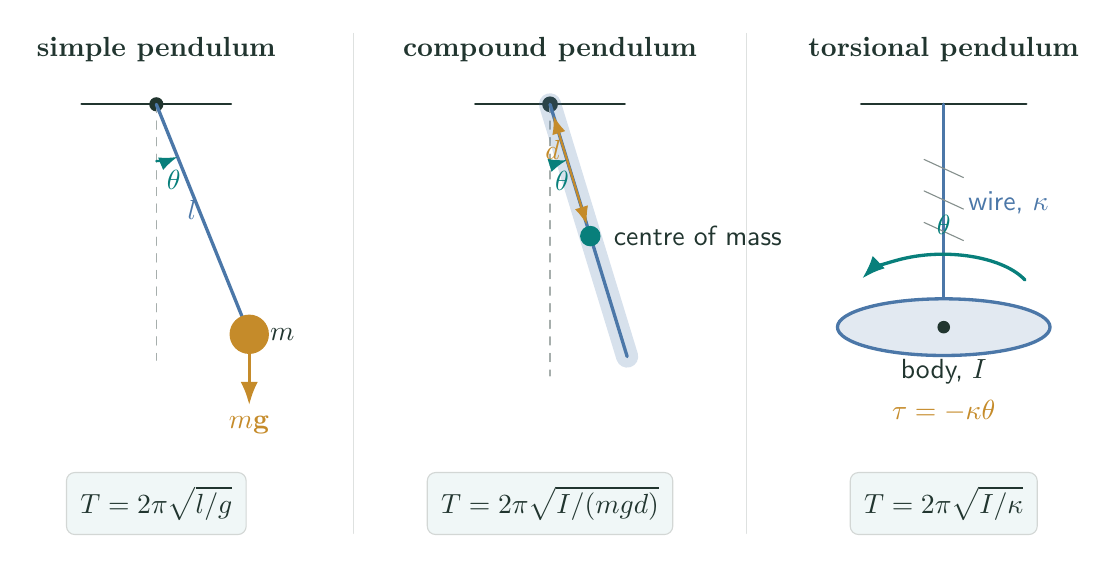
\begin{tikzpicture}[font=\sffamily,text=ink,>=Latex,line cap=round,line join=round]
  % Panel separators.
  \draw[ink!15] (3.0,-2.8)--(3.0,3.55);
  \draw[ink!15] (8.0,-2.8)--(8.0,3.55);

  % Simple pendulum.
  \node[font=\bfseries] at (0.5,3.35) {simple pendulum};
  \coordinate (P1) at (0.5,2.65);
  \coordinate (B1) at ($(P1)+(-68:3.15)$);
  \draw[ink,thick] (-.45,2.65)--(1.45,2.65);
  \fill[ink] (P1) circle (.09);
  \draw[ink!40,dashed] (P1)--++(0,-3.25);
  \draw[blue,very thick] (P1)--(B1) node[pos=.55,above left] {$l$};
  \fill[gold] (B1) circle (.25);
  \node[right=4pt] at (B1) {$m$};
  \draw[teal,thick,->] ($(P1)+(0,-.72)$)
    arc[start angle=-90,end angle=-68,radius=.72];
  \node[teal] at ($(P1)+(-77:.98)$) {$\theta$};
  \draw[gold,very thick,->] (B1)--++(0,-.9) node[below] {$m\mathbf g$};
  \node[draw=ink!20,rounded corners=3pt,fill=teal!6,inner sep=5pt]
    at (.5,-2.42) {$\displaystyle T=2\pi\sqrt{l/g}$};

  % Compound pendulum.
  \node[font=\bfseries] at (5.5,3.35) {compound pendulum};
  \coordinate (P2) at (5.5,2.65);
  \coordinate (C2) at ($(P2)+(-73:1.75)$);
  \coordinate (E2) at ($(P2)+(-73:3.35)$);
  \draw[ink,thick] (4.55,2.65)--(6.45,2.65);
  \fill[ink] (P2) circle (.10);
  \draw[ink!40,dashed] (P2)--++(0,-3.45);
  \draw[blue,very thick,line width=8pt,opacity=.22] (P2)--(E2);
  \draw[blue,very thick] (P2)--(E2);
  \fill[teal] (C2) circle (.13);
  \node[right=5pt] at (C2) {centre of mass};
  \draw[<->,gold,thick] ($(P2)+(-73:.15)$)--($(C2)+(-73:-.15)$)
    node[midway,above left] {$d$};
  \draw[teal,thick,->] ($(P2)+(0,-.74)$)
    arc[start angle=-90,end angle=-73,radius=.74];
  \node[teal] at ($(P2)+(-81:.98)$) {$\theta$};
  \node[draw=ink!20,rounded corners=3pt,fill=teal!6,inner sep=5pt]
    at (5.5,-2.42) {$\displaystyle T=2\pi\sqrt{I/(mgd)}$};

  % Torsional pendulum.
  \node[font=\bfseries] at (10.5,3.35) {torsional pendulum};
  \coordinate (P3) at (10.5,2.65);
  \draw[ink,thick] (9.45,2.65)--(11.55,2.65);
  \draw[blue,very thick] (P3)--(10.5,.15)
    node[midway,right=5pt] {wire, $\kappa$};
  \draw[ink!55,thin] (10.25,1.95)--(10.75,1.72);
  \draw[ink!55,thin] (10.25,1.55)--(10.75,1.32);
  \draw[ink!55,thin] (10.25,1.15)--(10.75,.92);
  \fill[blue!16] (10.5,-.18) ellipse (1.35 and .36);
  \draw[blue,very thick] (10.5,-.18) ellipse (1.35 and .36);
  \fill[ink] (10.5,-.18) circle (.08);
  \node at (10.5,-.18) [below=8pt] {body, $I$};
  \draw[teal,very thick,->]
    (11.53,.42) arc[start angle=24,end angle=154,x radius=1.14,y radius=.55];
  \node[teal,above] at (10.5,.87) {$\theta$};
  \node[gold] at (10.5,-1.25) {$\tau=-\kappa\theta$};
  \node[draw=ink!20,rounded corners=3pt,fill=teal!6,inner sep=5pt]
    at (10.5,-2.42) {$\displaystyle T=2\pi\sqrt{I/\kappa}$};
\end{tikzpicture}
\end{document}
